\documentclass[sigconf]{acmart}

\usepackage{hyperref}

\usepackage{endfloat}
\renewcommand{\efloatseparator}{\mbox{}} % no new page between figures

\usepackage{booktabs} % For formal tables

\settopmatter{printacmref=false} % Removes citation information below abstract
\renewcommand\footnotetextcopyrightpermission[1]{} % removes footnote with conference information in first column
\pagestyle{plain} % removes running headers

\begin{document}
\title{Big Data and Artificial Intelligence Solutions for in Home, Community and Territory Security}


\author{Ashok Reddy Singam}
\orcid{HID337}
\affiliation{%
  \institution{Indiana University}
  \streetaddress{711 N Park Ave}
  \city{Bloomington} 
  \state{Indiana} 
  \postcode{47408}
}
\email{asingam@iu.edu}

\author{Anil Ravi}
\orcid{HID333}
\affiliation{%
  \institution{Indiana University}
  \streetaddress{711 N Park Ave}
  \city{Bloomington} 
  \state{Indiana} 
  \postcode{47408}
}
\email{anilravi@iu.edu}

\begin{abstract}
Having an intelligent ear-and-eye monitoring system at the home to constantly observe the surroundings both inside and outside can protect the house and personnel much more safer way. By extending this capability to the neighborhood and city through collaboration would create safe cities across the world.

\end{abstract}

\keywords{i523, HID333, HID337, Artificial Intelligence, Natural Language Processing (NLP), Machine Learning, Micro Drone}

\maketitle

\section{Introduction}
For an application to be considered as big data application, volume has to be at least in the range of 30 to 50 terabytes. 
However, large volume alone is not an indicator of a big data problem. A small amount of data of different types, both structured and unstructured, that would also be considered as a big data problem. Since the Security Systems are going to generate continuous audio and video data, these applications fall under Big Data.

Here we are going to review existing systems, methods and research literature on security at various geographical levels to propose the improved systems implemented with artificial intelligence and big data infrastructure. Video surveillance of residential, commercial, military, and other restricted locations have been in practice since many years using various available technologies. 
Depending on the level of security, the data has been processed by data mining and/or big data analytics to take decisions by various personal, agencies and governments. 
However, the limitations of data collection, data mining and adoption of intelligence led to ineffective systems which are not predictive as they should be. 
Here we are proposing to use the integrated video and audio data of targeted regions (homes, public places and extended areas) along with social media data for analysis. 
The system uses advanced statistical methods, machine learning and classification algorithms to predict and prevent the threats based on the severity probability.

\subsection{Contemporary Security Systems}

The present security systems used by households are static cameras used at a fixed location inside or outside the house. They are connected to network and provide alerts when any event occurred. However, they are not intelligent enough to understand the context, recognizing the people faces, and aware of family members behaviors, house needs etc.

\subsection{Dynamic Video Analytics}

Video analytics plays a key role in modernizing video surveillance systems.Deep Learning the fastest growing field of Artificial Intelligence, enabling computers to interpret huge 
amounts of data like videos.A successful deep learning application requires a very large amount of data (thousands of images) to train the model, as well as GPUs, or graphics processing units, to rapidly process your data.The Graphics Processing Units (GPUs) provided by vendors like Nvidia enabling the deep learning infrastructure to cameras and recorders. The three most common ways people use deep learning to perform object classification are:

\begin{itemize}
 \item Training from Scratch
 \item Transfer Learning
 \item Feature Extraction
\end{itemize}

IntelliVision is one of the Video Analytics software currently in the market based on AI and Deep Learning for Smart Cameras, providing video analytics solutions for several markets including Smart Home/IoT, Security, Smart Retail, Smart Business, big data analytics and video search. 

\subsection{Live Voice Analytics}
Audio monitoring in addition to video helps false alarms by providing secondary verification.Traditional voice analytics tools rely on keywords and phonetics. These solutions are not well enough in deriving context and relevancy.With Big Data and AI advancements, now it is even possible to analyze for things like stress levels, lies, emotional content and more from audio data.Deep learning is becoming a mainstream technology for speech recognition and has successfully replaced  Gaussian  mixtures  for  speech  recognition  and  feature  coding  at  an  increasingly  larger scale. Google's Speech Recognition api  built using deep learning neural network algorithms is one of the voice analytics software available in the market.

\section{Big Data Infrastructure}
Big Data applications requires huge storage and computing power.Big Data organizes and extracts the valued information from the large volumes, variety forms and frequently changing data sets collected from multiple, and autonomous sources 
in the minimal possible time, using several mathematical and machine learning techniques.

A big data solution typically comprises these logical layers:
 \begin{itemize}
    \item Big data sources: Text,Audio,Video etc
    \item Data massaging and store layer: This layer is responsible for acquiring data from the data sources and, if necessary, converting it to a format that suits how the data is to be analyzed. 
    Ex:Hadoop Distributed File System (HDFS) store
    \item Analysis layer:The analysis layer reads the data digested by the data massaging and store layer.For example, this layer offers tools like NoSQL programming, and Map Reduce for data intensive computing, domain specific statistical models, machine learning techniques etc
    \item Consumption layer:This layer consumes the output provided by the analysis layer. The consumers can be visualization applications, human beings, business processes, or services
 \end{itemize}
 
\begin{figure}
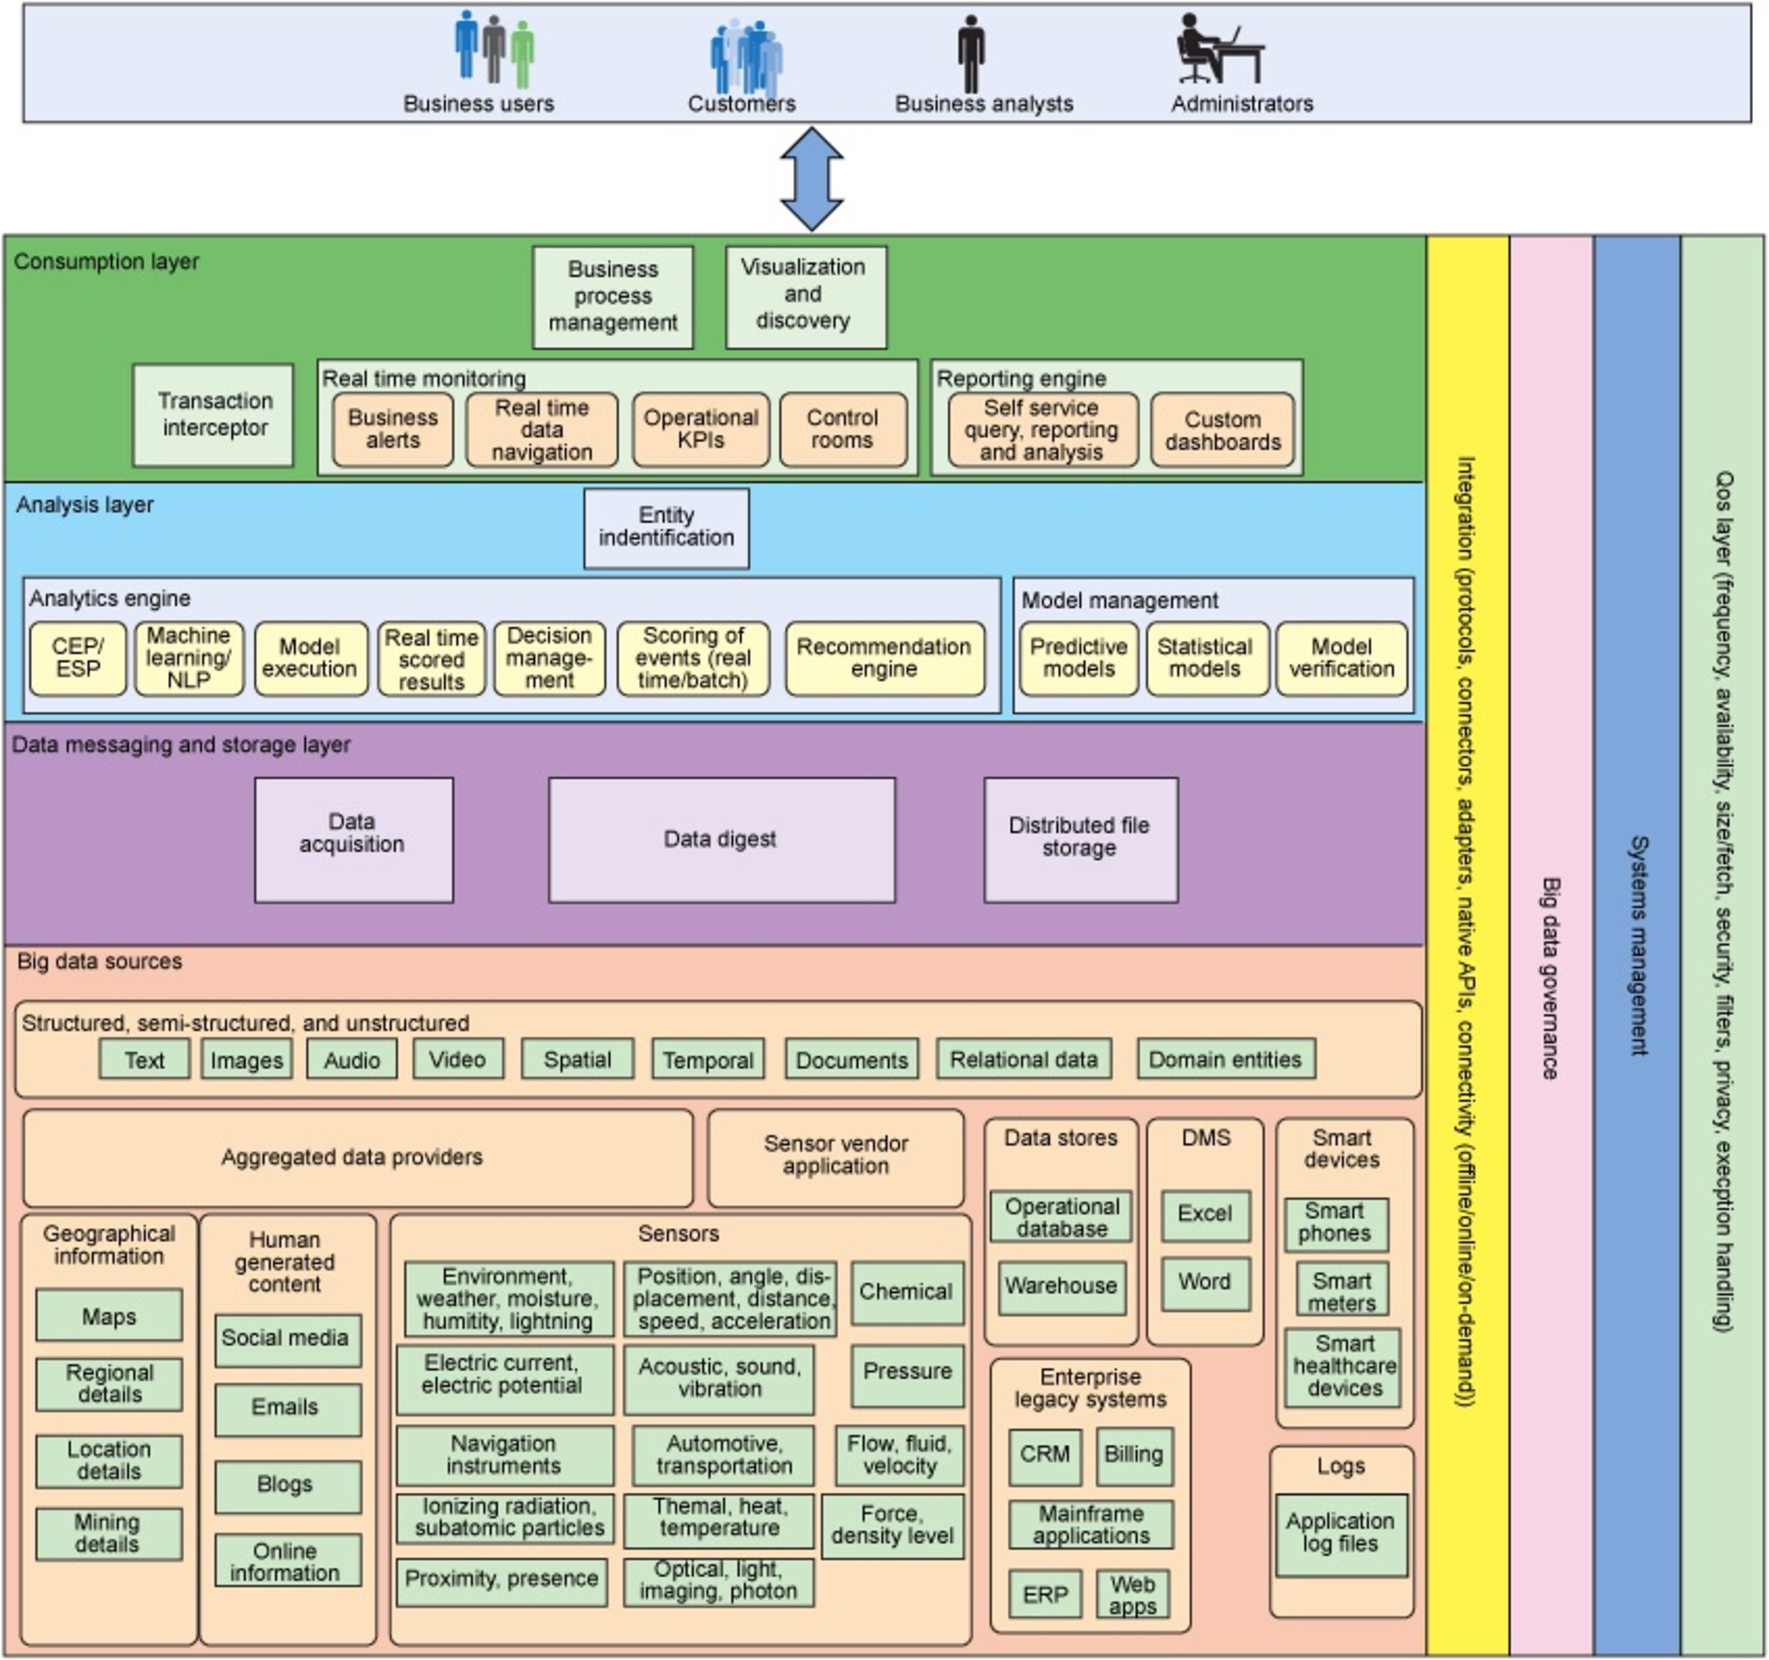
\includegraphics[height=8in, width=7.5in]{images/BigDataArchitecture.pdf}
\caption{Typical Big Data Architecture}
\end{figure}
 
\section{Home Security}

\section{Community/Regional Security}

\section{Extended Regional Security}

\section{Conclusions}
In the today's technology world, drones are becoming more familiar in the main stream life activities such as recreational, spy cameras by authorities, home delivery of goods etc.

By making cameras movable across the house and outside and process the data as humans do and take decisions of alerting or informing to the right people is the key concept of this paper.This system to be functional, the following technologies needed:

\begin{itemize}
  
\item Micro drones with audio and video sensors

\item Facial recognition and mapping through video analytics to recognize people
	
\item Natural language processing (NLP) to recognize family members, friends and strangers

\item Machine learning algorithms to understand family members habits and behaviors

\item Interfacing with email servers, phone, text message servers

\end{itemize}

\begin{acks}
The authors would like to thank professor Gregor von Laszewski and his team for providing LaTex templates
\end{acks}

\bibliographystyle{ACM-Reference-Format}
\bibliography{report} 

\end{document}
